\documentclass[UTF8,12pt]{ctexart}
\usepackage{amsmath,amssymb,geometry,bm,graphicx,fontspec,amssymb,amsthm}
\usepackage[mathscr]{euscript}

\usepackage[colorlinks,
linkcolor=black,
anchorcolor=blue,
citecolor=green
]{hyperref} % 目录中的超链接

%数学定理
\newtheorem{Def}{定义}[section]
\newtheorem{Theo}{定理}[section]
\newtheorem{Lemm}{引理}[section]
\newtheorem{Prop}{命题}[section]
\newtheorem{Assu}{假设}[section]
\newtheorem{Axiom}{Axiom}

\newenvironment{Dr}{\noindent 借:}{\par}
\newenvironment{Cr}{\noindent 贷:}{\par}

\numberwithin{equation}{section} % 按章节进行排序与编号
\numberwithin{figure}{section}
\numberwithin{table}{section}

\usepackage{draftwatermark} % 所有页加水印
\SetWatermarkText{EconNerd} % 设置水印内容
\SetWatermarkLightness{0.99} % 设置水印透明度 0-1
\SetWatermarkScale{1} % 设置水印大小    

\title{CPA} % 文档相关信息
\author{EconNerd}
\date{\today}
\geometry{scale=0.8}

\begin{document}
	\maketitle
	\tableofcontents
	\newpage
	
	\section{基础知识}
	
	会计科目众多分可为四类,资产负债类、损益类、所有者权益类、成本类。
	
	损益类科目:主营业务成本、其他业务成本、税金及附加、销售费用、管理费用、财务费用、资产减值损失、信用减值损失、营业外支出、所得税费用。
	
	主营业务收入、其他业务收入、公允价值变动损益、投资收益、资产处置损益、其他收益、营业外收入、以前年度损益调整。除了以前年度损益调整外的所有科目就是\textbf{当期损益}。
	
	\subsection{利率相关}
	在利率中经常出现年金现值系数(P/A)和复利现值系数(P/F).
	
	其中P代表现在,F代表未来,A代表年金。通常这些系数都会给出。结合终值,我们就可以计算出现值。
	
	\subsection{每章和费用相关}
	无形资产开发中的费用化计入管理费用
	
	\begin{Dr}
		固定资产 \par
		无形资产
	\end{Dr}
	\begin{Cr}
		银行存款
		
		应付票据
	\end{Cr}
	
	\newpage
	
	\section{存货}
	\subsection{存货的确认和初始计量}
	\paragraph{什么是存货} 
	\textit{存货的概念}:日常活动中\textbf{持有以备出售}的。 
	\textit{确认条件}:1.经济利益很可能流入企业 2.可以可靠计量
	
	\paragraph{初始计量}
	总体来说以\textbf{成本}进行计量,根据取得方式不同采用不同的计量方式。(\textbf{包括低值易耗品},\textbf{合理损耗计入成本},\textbf{季节性停工的制造费用计入成本},入库无发票或发票无入库都算存货,摊销期不超过一年的确认为资产的合同履约成本,生产成本余额,以发出但不符合收入确认条件的存货)
	
	不同的取得方式:
	\begin{enumerate}
		\item 外购所得。外购成本包括\textbf{购买价款}、\textbf{相关税费}(不可抵扣的税费)、\textbf{其他相关费用}(入库前的合理损耗)。\textbf{商品流通企业}进货\textbf{金额较小}可以直接计入\textbf{当期损益}(销售费用)
		
		\item 加工所得。存货的加工成本,包括直接人工以及按照一定方法分配的制造费用。
		
		\item 其他方式。收投资者投资,按照公允价值入账,差额计资本溢价或股本溢价。剩余方式按照其他准则来确定。
		
		\item 劳务取得。劳务人员的直接人口和其他费用计入成本。
	\end{enumerate}
	
	\paragraph{确认损益,不计入成本的情况}
	\begin{enumerate}
		\item 非正常消耗的直接材料、直接人工和制造费用。运输过程中因自然灾害发生的损失。
		
		\item 存货在采购入库后领用前所发生的仓储费用,应计入当期损益(管理费用)
		
		\item 不能归属于使存货达到目前场所和状态的其他支出
		
		\item 企业采购用于广告营销活动的特定商品,向客户预付货款未取得商品时,应作为预付账款进行会计处理,待取得相关商品时计入当期损益(销售费用)。企业取得广告营销性质的服务比照该原则进行处理 
	\end{enumerate}
	
	\subsection{发出存货的计量}
	\paragraph{发出的计量} 发出的计量主要有四种不同的方法:先进先出、移动加权平均、月末一次加权平均、个别计价法。
	\begin{enumerate}
		\item 先进先出。字面意思。
		
		\item 移动加权平均。每次进货计算成本,加权计算存货的成本来运用到下次进货前发出存货中。
		
		\item 月末一次加权平均。月末计算成本,以库存和本月来进行加权计算,并运用到本月的发出存货中。
		
		\item 个别计价法。字面意思。
	\end{enumerate}
	
	\paragraph{成本的结转} 有几种不同的情况,会计分录如下
	\begin{enumerate}
		\item 对外销售商品,结转成本。借:主营业务成本、存货跌价准备。贷:库存商品
		
		\item 对外销售材料,结转成本。借:其他业务成本、存货跌价准备。贷:原材料
		
		\item 包装物的会计处理。生产领用的计入\textbf{制造费用};出借或不单独计价的计入\textbf{销售费用};出租或单独计价的计入\textbf{其他业务成本}。
	\end{enumerate}
	
	\subsection{期末存货的计量}
	期末存货与可变现净值进行比较,若小于可变现净值,则需要计提存货跌价准备,并计入当期损益。
	
	\paragraph{期末计量}
	如果\textbf{存货直接售卖},则按\textbf{有无合同}进行区分。无合同则按市场价计算,有合同在合同数量内的按合同价计算,合同外的数量按市场价计算。\textbf{两部分分开算跌价准备}
	
	\textbf{材料直接出售},可变现净值为预计售价-相关销售费用和税费。
	
	\textbf{材料用于生产},则需要看\textbf{最终产品是否发生减值}。不发生减值则不做处理,发生减值则需要按照可变现净值进行处理,且可变现净值为估计售价-达到产品状态所需成本-相关销售费用和税费。
	
	\paragraph{跌价准备} 主要涉及计提、转回和结转三个方面。
	
	可变现净值较低时就需要计提跌价准备,通常按照单个存货项目计提。种类繁多、单价较低可以按照类别进行计提。计提的存货跌价准备应当计入当期损益(资产减值损失)。
	
	当以前减计存货价值的影响因素消失时,可以在已计提的跌价准备金额内转回,转回金额计入当期损益。
	
	结转方面,存货跌价准备结转至主营业务成本或其他业务成本。此时存货已经销售。
	
	\subsection{存货的清查盘点}
	
	主要分为盘盈与盘亏,还要考虑所得税的因素。无论盘盈还是盘亏,首先都要通过“待处理财产损溢”科目。
	
	\paragraph{盘盈} 批准前按照\textbf{重置成本}作为入账价值,并通过“待处理财产损溢”科目进行会计处理。批准后冲减管理费用。
	
	\paragraph{盘亏} 盘亏可能存在着不同的原因,但是在批准前都是计入“待处理财产损溢”科目。
	\begin{enumerate}
		\item 自然灾害等非常原因。残料入库计原材料、残料变现计银行存款、应收的赔款计其他应收款、差额计入\textbf{营业外支出}。
		
		\item 计量收发差错和管理不善。残料入库计原材料、残料变现计银行存款、应收的赔款计其他应收款、差额计入\textbf{管理费用}。
		
	\end{enumerate}
	
	\paragraph{增值税相关}
	因\textbf{管理不善}或\textbf{违反法律}造成的盘亏,不能抵扣的进项税额应当转出。
	
	\newpage
	\section{固定资产}
	\textit{固定资产的概念}:使用寿命\textbf{超过一个会计年度}的,为生产商品等目的而持有的。
	
	\subsection{确认和初始计量}
	
	整体来说,固定资产当按照\textbf{取得成本}进行初始计量。
	
	取得成本为\textbf{达到预定可使用状态}前所发生的所有合理必要的支出,如借款利息资本化的部分。根据取得方式不同有着不同的成本计算。
	
	\begin{enumerate}
		\item \textit{外购固定资产}。如果需要\textbf{安装},先计入在建工程,最后转入固定资产。不需要安装则直接转入固定资产。如果\textbf{一次购买了多个}固定资产,则将成本以公允价值进行分配。
		
		企业购买固定资产的价款超过正常信用条件延期支付,实质上具有\textbf{融资性质}的.固定资产的成本以\textbf{购买价格的现值为基础确定} 。 实际支付的价款与购买价款的现值之间的差额,采用\textbf{实际利率法进行摊销}。满足资本化计入成本,其他计入损益(财务费用)。
		
		简单来说,如果以融资方式购买了1000万的资产,那么虽然公司在未来的几期内总共支付了1000万,但是其中并不是所有都算入成本,而是有一部分算入利息。
		
		因此在入账的时候要区分所有的支付款(长期应付款)和利息(未确认融资费用)。在每次支付款项的时候都进行利息的摊销。
		
		\item \textit{自营方式自行建造}的固定资产。以直接材料、直接人工等进行计量。
		\begin{figure}[htp]
			\centering
			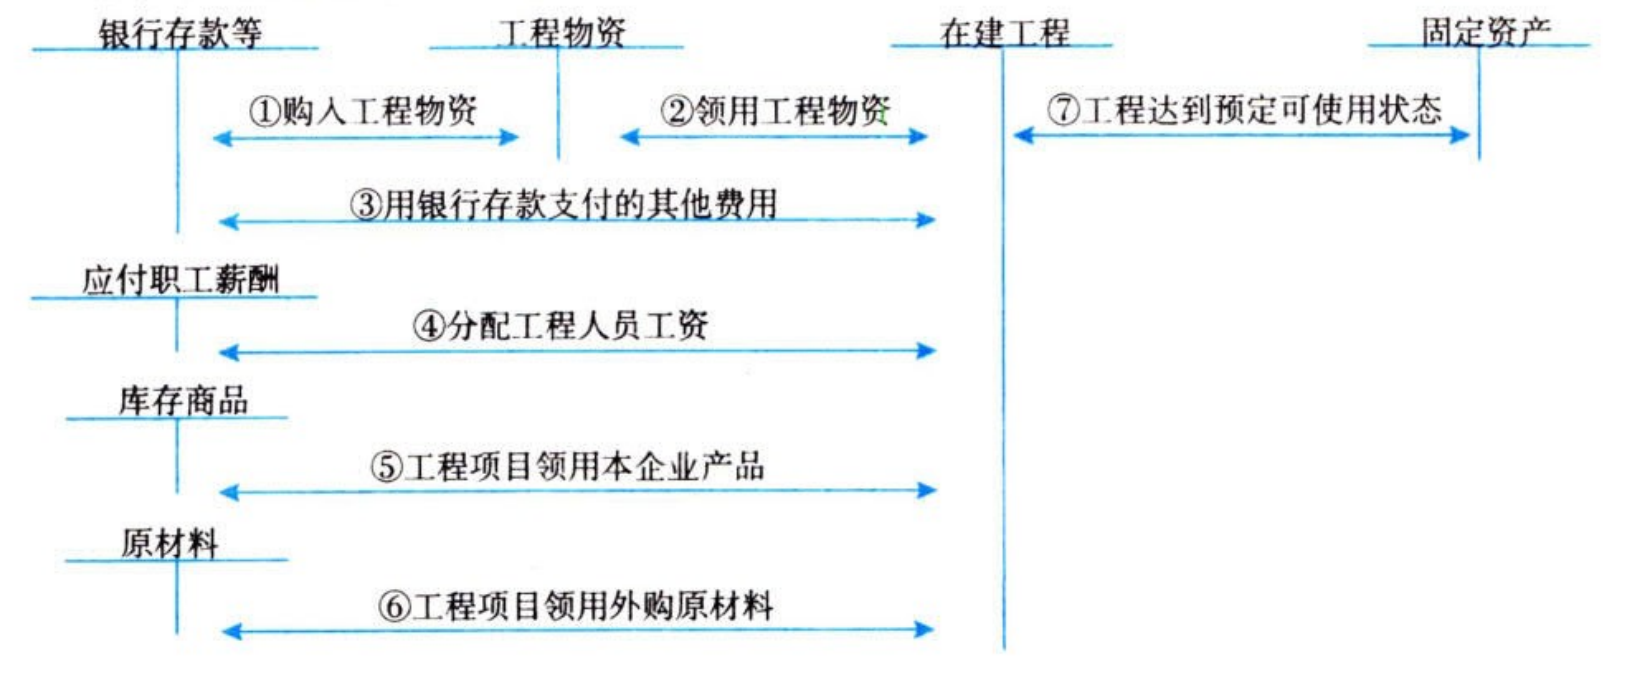
\includegraphics[width=1\linewidth]{pic/3.1.png}
			\caption{Caption}
			\label{fig:enter-label}
		\end{figure}
		
		\textbf{建设期间}盘亏、报废、损坏计入成本;盘盈冲减成本。完工后计入\textbf{当期损益}。
		
		\textbf{已达到预定可使用状态,但尚未办理竣工的}。以暂时估值转入固定资产,并计提折旧。办理竣工后调整估值,但是\textbf{不调整已经计提的折旧}。
		
		\item 出包方式建造固定资产。出包方式建造中有额外的一项待摊支出。\textbf{待摊支出}是指在建设期间发生的,\textbf{不能直接计入某项固定资产价值}、而应由所建造固定资产共同负担的相关费用。
		
		\textbf{待摊支出分配率}=累计发生的待摊支出/(建筑工程支出+安装工程支出+在安装设备支出 )
		
		A工程\textbf{应分配的待摊支出}=(A工程的建筑工程支出+A工程的安装工程支出+A工程的在安装设备支出)* 待摊支出分配律
		\begin{figure}[htp]
			\centering
			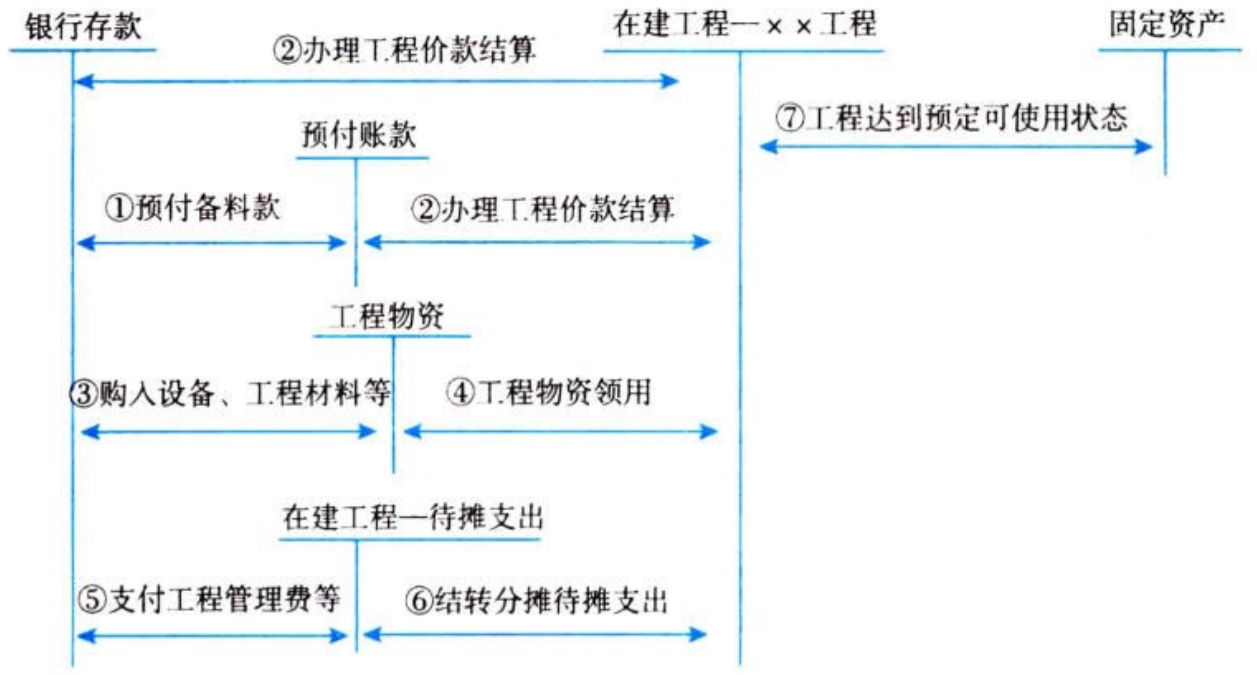
\includegraphics[width=1\linewidth]{pic/3.2.png}
			\caption{Caption}
			\label{fig:enter-label}
		\end{figure}
		
	\end{enumerate}
	
	保险费用如何计量?
	
	设备维修费用如何计量?
	
	高危行业需要提取安全生产费,处理如下
	
	\textbf{提取安全生产费时}
	
	借:生产成本、制造费用(或当期损益)
	
	贷:专项储备
	
	\textbf{使用提取的安全生产费时,费用性支出}
	
	借:专项储备
	
	贷:银行存款
	
	\textbf{形成固定资产的支出}
	
	发生支出时
	
	借:在建工程
	
	贷:银行存款或应付职工薪酬
	
	达到预定可使用状态
	
	借:固定资产
	
	贷:在建工程
	
	借:专项储备
	
	贷:累计折旧(按照固定资产入账金额一次性计提折旧)
	
	
	
	\subsection{后续计量}
	固定资产的后续计量主要包括两方面:固定资产的\textbf{折旧}、固定资产的\textbf{后续支出}。
	
	\subsubsection{折旧}
	注意事项:1.转入在建工程后不计提折旧2.大修期间计提折旧3.季节性修理需要计提折旧4.达到可使用状态前的出售产品,试验计入成本。
	
	折旧方法主要包括年限平均法、工作量法、双倍余额递减法和年数总和法。折旧方法确定后不得随意更改。
	
	\begin{enumerate}
		\item 年限平均法。以年来平均提折旧。
		
		\item 工作量法。以工作量来平均提折旧。
		
		\item 双倍余额递减法。年折旧额=期初固定资产净值*2/预计使用年限。最后两年改为年限平均法。
		
		\item 年数总和法。年折旧额=(原价-预计净残值)*年折旧额。年折旧额=年数之和做分母,年数倒转顺序作为分子
	\end{enumerate}
	
	会计处理为:
	
	借:制造费用(生产车间计提折旧)、管理费用、销售费用、其他业务成本、研发支出、在建工程。
	
	贷:累计折旧
	
	~\
	
	固定资产在后期可能会进行更新改造或修理,存在后续支出。资本化的后续支出计入成本,并将被替换部分的账面价值扣除。会计分录为
	
	固定资产账面价值\textbf{转入在建工程}
	
	借:在建工程、累计折旧、固定资产减值准备
	
	贷:固定资产
	
	\textbf{扣除被替换部分价值}
	
	借:银行存款、营业外支出(差额)
	
	贷:在建工程
	
	发生资本化\textbf{后续支出}
	
	借:在建工程
	
	贷:应付职工薪酬、原材料等
	
	\textbf{达到预定可使用状态}
	
	借:固定资产
	
	贷:在建工程
	
	费用化的后续支出计入当期管理费用或销售费用。
	
	
	\subsection{处置}
	
	处置包括固定资产的出售、转让、报废或损毁、对外投资、非货币性资产交换、债务重组等。
	\begin{figure}[htp]
		\centering
		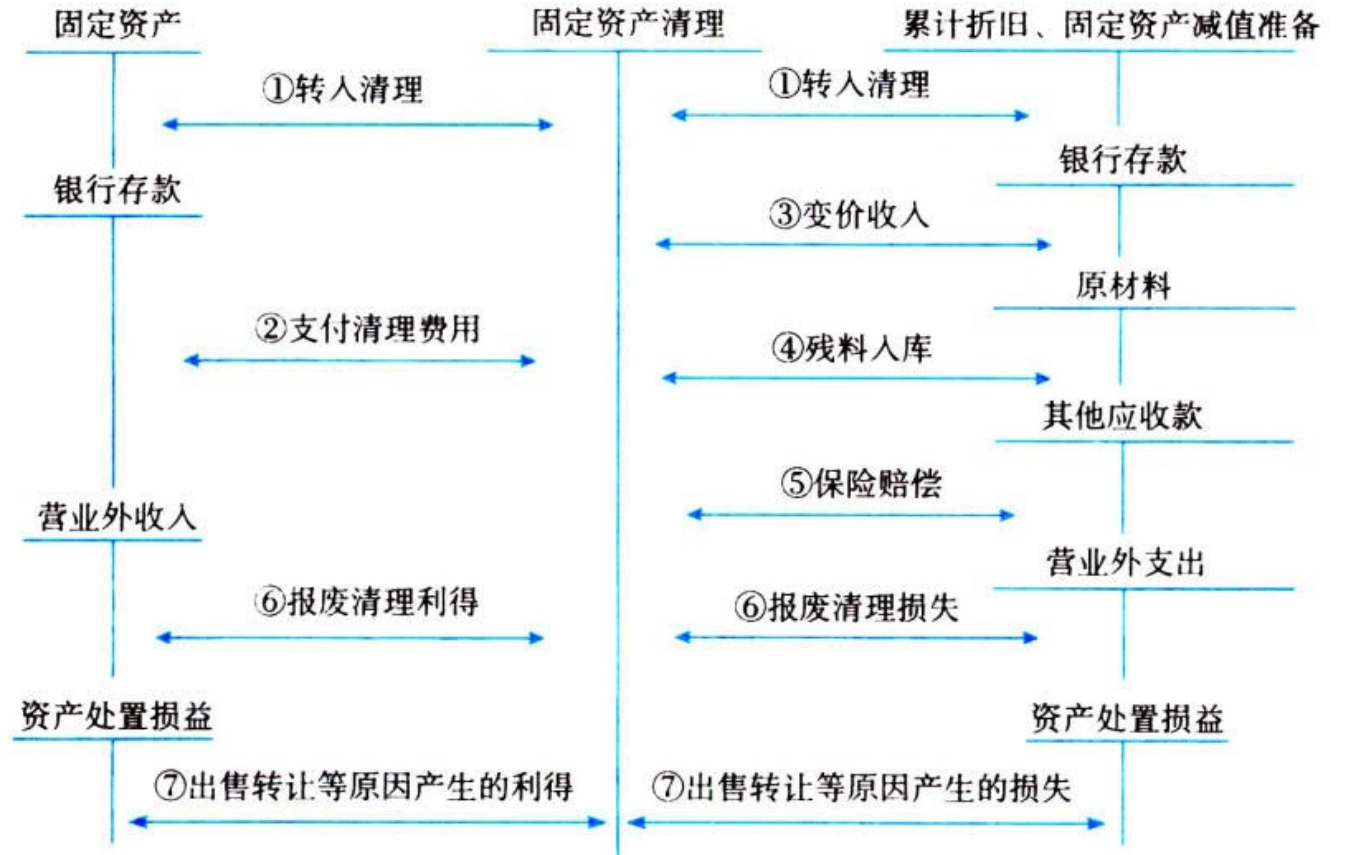
\includegraphics[width=1\linewidth]{pic/3.3.png}
		\caption{Caption}
		\label{fig:enter-label}
	\end{figure}
	
	固定资产的处置方式不同,适用不同的处理方法。
	\begin{enumerate}
		\item 生产期间正常报废清理,借:营业外支出-非流动资产报废,贷:固定资产清理
		
		\item 自然灾害造成的,借:营业外支出-非常损失,贷:固定资产清理
		
		\item 因出售或转让产生的利得或损失计入资产处置损益,产生净损失的,借:资产处置损益,贷:固定资产清理
	\end{enumerate}
	
	\subsubsection{固定资产的清查}
	清查可能出现盘盈或盘亏。
	
	盘盈情况下作为前期差错处理。借:固定资产(重置成本),贷:以前年度损益调整。
	
	盘亏情况计入营业外支出
	\begin{figure}[htp]
		\centering
		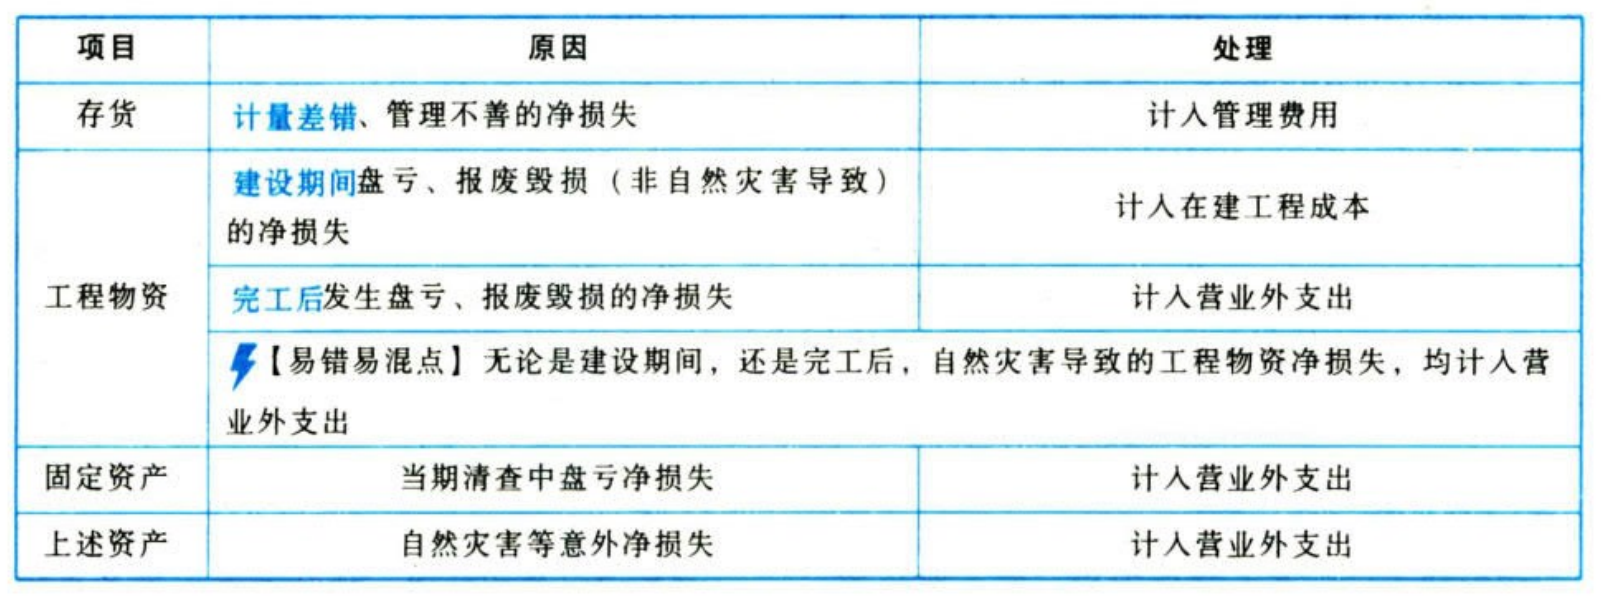
\includegraphics[width=1\linewidth]{pic/3.4.png}
		\caption{Caption}
		\label{fig:enter-label}
	\end{figure}
	
	
	
	\newpage
	\section{无形资产}
	
	无形资产:没有实物形态的可辨认货币性资产。主要包括专利权、非专利技术、商标权、著作权、土地使用权、特许权等。
	
	\subsection{确认与初始计量}
	
	按照实际成本进行初始计量。不同的取得方式有着不同的计量方法。
	\begin{enumerate}
		\item 外购获得。达到预定可使用状态前的费用。具有融资性质的,以现值为基础进行摊销,需要摊销。
		
		\item 投资者投入。根据投资合同或协议确定成本。
		
		\item 非货币性资产交换、债务重组。根据另外两个细分准则进行确定。
		
		\item 政府补助。按公允价值进行计量。无公允价值按照名义金额。
		
		\item 土地使用权。可能作为不同的资产进行核算。固定资产、无形资产、投资性房地产、存货。
	\end{enumerate}
	
	\subsection{内部研究开发支出的确认和计量}
	研发支出可以可能资本化计入无形资产,也可能费用化计入管理费用。
	
	一般来说开发阶段支出进行资本化、研究阶段以及无法资本化的开发阶段支出进行费用化。如果无法区分两个阶段则全部计入管理费用。
	
	\subsection{后续计量}
	后续计量主要考虑摊销,分为寿命确定与不确定两种情况。
	
	\textbf{寿命确定}的情况下需要进行摊销,方法与经济利益预期消耗方式有关。摊销一般计入当期损益,如果用于生产产品则会计入生产成本或制造费用。
	
	\textbf{寿命不确定}的情况下需要在每期期末进行减值测试。
	
	这里需要注意无形资产摊销和固定资产折旧的\textbf{区别}。无形资产摊头不摊尾,固定资产摊尾不摊头。
	
	\subsection{处置}
	
	处置主要包括三种情况:出售、出租、报废。
	
	\subsubsection{出售}
	差额计入\textbf{资产处置损益}。
	
	借:银行存款、
	无形资产减值准备、
	累计摊销
	
	贷:无形资产、
	应交税费-应交增值税(销项税额)、
	资产处置损益
	
	\subsubsection{出租}
	
	\textbf{确认收入}
	
	借:银行存款
	
	贷:其他业务收入、应交税费-应交增值税(销项税额)
	
	\textbf{相关费用计入成本}
	
	借:其他业务成本
	
	贷:累计摊销、银行存款
	
	\subsubsection{报废}
	
	不能带来价值,以账面价值\textbf{计入当期损益}
	
	借:营业外支出、累计摊销、无形资产减值准备
	
	贷:无形资产
	
	\newpage
	\section{投资性房地产}
	
	投资性房地产:为\textbf{赚取租金}或\textbf{资本增值}而持有的房地产。
	
	主要包括已出租的土地使用权(计划但尚未的不算)、持有并准备增值后转让的土地使用权、已出租的建筑物(转租不算、管理层决定出租的也算)。
	
	房地产可以有很多用途,如果无法区分则不确认为投资性房地产。
	
	\subsection{确认与初始计量}
	
	投资性房地产按成本计量。不同方式有着不同的计量方式。
	
	\begin{enumerate}
		\item 外购。外购直接用于投资和增值则计入无形资产,否则先计入固定资产和无形资产,后续开始租赁或用于增值则转换为投资性房地产。
		
		\item 自行建造。非正常损失计入当期损益,不计入建造成本。
	\end{enumerate}
	
	后续支出满足资本化的计入成本,在改扩建期间不进行折旧或摊销。后续费用化的支出计入当期损益(其他业务成本)。
	
	\subsection{后续计量}
	投资性房地产的后续计量可以分为\textbf{成本模式}或\textbf{公允价值模式}。两者的科目设置不同,会计处理也不同。
	
	\subsubsection{成本模式}
	成本模式下科目为:投资性房地产、投资性房地产累计折旧(摊销)、投资性房地产减值准备。会计处理如下。
	
	1.计提折旧或摊销
	
	借:其他业务成本
	
	贷:投资性房地产累计折旧(摊销)
	
	2.计提减值准备
	
	借:资产减值损失
	
	贷:投资性房地产减值准备
	
	3.取得租金收入
	
	借:银行存款
	
	贷:其他业务收入、应交税费-应交增值税(销项税额)
	
	值得注意的是,投资性房地产中土地使用权与建筑物的折旧和摊销和无形资产与固定资产的摊销方式相同。
	
	\subsubsection{公允价值模式}
	只有公允价值可以可靠获得时才可以使用公允价值模式。
	
	科目设置:投资性房地产-成本、投资性房地产-公允价值变动、公允价值变动损益。
	
	1.公允价值上升
	
	借:投资性房地产-公允价值变动
	
	贷:公允价值变动损益
	
	2.公允价值下降
	
	借:公允价值变动损益
	
	贷:投资性房地产-公允价值变动
	
	3.取得租金收入
	
	借:银行存款
	
	贷:其他业务收入,应交税费-应交增值税
	
	\subsubsection{模式改变}
	可以由成本模式转为公允价值模式,反之不行。此时作为会计政策变更处理,根据公允价值与账面价值的差额调整期初留存收益。会计处理如下。
	
	借:投资性房地产(变更日公允价值)、投资性房地产累计折旧(摊销)投资性房地产减值准备
	
	贷:投资性房地产(原价)、利润分配-未分配利润、盈余公积(或借方)
	
	\subsection{转换与处置}
	\subsubsection{转换}
	转换上可能存在“自动房地产与存货”和“投资性房地产”之间的转换。
	
	在成本模式下,两者之间按照账面价值进行互相转换。
	
	公允价值模式下,投资性房地产转非投资性,差额计入公允价值变动损益。非投资性转投资性,借方差额计入公允价值变动损益,贷方差额计入其他综合收益。
	
	\subsubsection{处置}
	\paragraph{成本模式下}
	
	\textbf{1.确认收入}
	
	借:银行存款
	
	贷:其他业务收入、应交税费-应交增值税(销项税额)
	
	\textbf{2.确认成本}
	
	借:其他业务成本、投资性房地产累计折旧、投资性房地产减值准备
	
	贷:投资性房地产
	
	\paragraph{公允价值模式下}
	\textbf{1.确认收入}
	
	借:银行存款
	
	贷:其他业务收入、应交税费-应交增值税
	
	\textbf{2.确认成本}
	
	借:其他业务成本
	
	贷:投资性房地产-成本、-公允价值变动
	
	借:其他综合收益
	
	贷:其他业务成本
	
	借:公允价值变动损益
	
	贷:其他业务成本
	
	\newpage
	\section{长期股权投资与合营安排}
	\subsection{基本概念}
	首先对外投资来说可以分为股权投资和其他投资。而股权投资又包括了长期股权投资以及《金融工具确认与计量》所规定的股权投资。
	
	只有投资方对被投资方实施控制、重大影响的权益性投资才能被叫做长期股权投资。
	
	\subsection{初始计量}
	
	
	\newpage
	\section{资产减值}
	主要内容:什么是资产减值、资产可收回金额的计量、资产减值损失的确认和计量、资产组的认定及减值处理、商誉减值测试与处理
	
	\subsection{资产减值概述}
	\paragraph{什么是资产减值}资产减值是指资产的可收回金额低于其账面价值(账面余额减备抵项目)。整体思路和存货的跌价准备类似。
	
	但是资产减值使用范围是8号准则,主要适用于\textbf{非流动资产}。具体来说包括
	\begin{enumerate}
		\item 对子公司(控制)、联营企业(重大影响)和合营企业(共同控制)的长期股权投资
		
		\item 成本模式后续计量的投资性房地产
		
		\item 固定资产
		
		\item 生产性生物资产
		
		\item 无形资产
		
		\item 商誉
		
		\item 探明石油天然气矿区权益和井及相关设施 
	\end{enumerate}
	
	资产减值要在资产负债表日判断资产是否存在可能发生减值的迹象。如果存在减值几项,应当进行减值测试,估计资产的可收回金额。可收回金额低于账面价值的应当按照可收回金额低于账面价值的差额计提减值准备,确认减值损失。
	
	\paragraph{特殊情况}资产减值还存在着以下三种特殊情况,无论如何至少每年需要进行减值测试:
	\begin{enumerate}
		\item 因企业合并所形成的商誉
		
		\item 使用寿命不确定的无形资产
		
		\item 对于尚未达到预定用途的无形资产(研发支出-资本化支出:因其价值通常有较大不确定性)
	\end{enumerate}
	
	企业存在以下情况的,可以不估计其可收回金额:
	\begin{enumerate}
		\item 前报告期间的计算结果表明,资产可收回金额远高于其账面价值,之后又没有发生消除这一差异的交易或者事项的,企业在资产负债表日可以不需重新估计该资产的可收回金额。
		\item 以前报告期间的计算与分析表明,资产可收回金额对于资产减值准则中所列示的一种或者多种减值迹象反应不敏感(出现的减值迹象对本企业没有影响),在本报告期间又发生了这些减值迹象的,在资产负债表日企业可以不需因为上述减值迹象的出现而重新估计  该资产的可收回金额。
	\end{enumerate}
	
	\subsection{资产可收回金额的计量}
	什么是资产可收回金额:公允价值减处置费用和未来现金流量现值两者的\textbf{较高值}。(为数不多的较高者)
	
	资产可收回金额存在着以下特殊情况:
	\begin{enumerate}
		\item 资产的公允价值减去处置费用后的净额与资产预计未来现金流量的现值,只要有一项超过了资产的账面价值,就表明资产没有发生减值,\textbf{ }。
		\item 没有确凿证据或者理由表明,资产预计未来现金流量现值显著高于其公允价值减去处置费用后的净额,可以\textbf{将资产的公允价值减去处置费用后的净额视为资产的可收回金额}。(如:持有待售的非流动资产)
		\item 资产的公允价值减去处置费用后的净额如果无法可靠估计的,应当以该\textbf{资产预计未来现金流量的现值作为其可收回金额}。
		
	\end{enumerate}
	
	\subsubsection{资产公允价值减去处置费用}
	处置费用是指可以直接归属于资产处置的增量成本,包括与资产处置有关的法律费用、相关税费、搬运费以及为使资产达到可销售状态所发生的直接费用。但是财务费用(筹资活动不是经营活动)和所得税费用(我们用的是税前的金额)不包括在内。
	
	公允价值应当按照以下顺序进行:
	\begin{enumerate}
		\item 公平交易中资产的销售协议价格(有协议)
		
		\item 该资产的市场价格(无协议,市场价)
		
		\item 熟悉情况的交易双方资源进行公平交易愿意提供的交易价格(无协议、无市场)
	\end{enumerate}
	以上三种情况都不存在,则公允价值无法可靠估计,按照未来现金流量的现值进行估计
	
	\subsubsection{未来现金流量的现值}
	考虑持续使用过程中和最终处置时产生的现金流量。因此考虑因素包括三个:\textbf{资产的预计未来现金流量}(现金流入、流出、处置资产得到的现金流量)、\textbf{资产的预计使用寿命}、\textbf{折现率} (计算难度大于未来现金流量,因此宁可确认公允价值减处置费用)
	
	预测现金流量应在剩余使用寿命内,最多涵盖5年,除非存在更多证据,可以进行延长。
	
	在建工程和开发中的无形资产,还需要考虑达到预定可使用状态的现金流出。
	
	接下来我们考虑如何预计资产未来现金流量。预计资产未来现金流量需要考虑以下因素
	\begin{enumerate}
		\item 以资产当前状况为基础预计资产未来现金流量。不考虑未来可能发生、尚未做出承诺的重组事项或资产改良相关的未来现金流量。
		
		已经承诺重组的,应当反应重组所节约的费用或者其他利益,以及相关的未来现金流出数。
		
		\item 预计未来现金流量不应当包括筹资活动和所得税收付产生的现金流量(不包括财务费用与所得税,和公允价值方法类似)
		
		\item 对通货膨胀的考虑应当与折现率一致
		
		\item 内部转移价格应当予以调整
	\end{enumerate}
	
	预计资产未来现金流量有两种方法
	\begin{enumerate}
		\item 传统法:根据资产未来每期最有可能产生现金流量进行预测
		
		\item 期望现金流量法:概率加权平均
	\end{enumerate}
	
	针对折现率,也有不同的预计方法。 
	\begin{enumerate}
		\item 由于现金流量也是税前的概念,因此折现率也是税前利率。折现率时企业在购置或者投资资产时所要求的必要报酬率。
		
		\item 企业确定这些率时,应当以该资产的市场利率作为依据,无法获得时使用替代利率。(加权平均资金成本、增量借款利率或者其他相关市场借款利率作适当调整后确定)
		
		\item 通常使用单一折现率,如果未来现金流量现值对不同旗舰的风险差异或者利率的期限结构反应敏感,企业应当采用不同的折现率。 
	\end{enumerate}
	
	当存在外币的未来现金流量时,遵循原则(先折现、后折算),按照当日的即期汇率进行折算
	
	\subsection{资产减值损失的确认与计量}
	资产可收回金额低于账面价值,计提资产减值损失,计入当期损益,同时计提相应的资产减值准备。
	
	资产减值损失确认后,资产的折旧或摊销应在未来旗舰作相应调整。
	
	\paragraph{关于转回}
	资产减值损失确认一经确认,在以后会计期间\textbf{不得转回}。以前期间计提的资产减值准备,需要等到资产处置时才可转出。(准备减少记方)
	
	可以转回的占少数(存货跌价准备,对应的信用减值损失(22号准则(金融工具的减值)坏账准备、债券投资减值准备、综债、应收融资租赁款),递延所得税资产发生减值,持有待售的减值准备)
	
	合同资产减值准备用的对应科目是资产减值损失,原本用的信用减值损失,也可以转回。 
	
	\paragraph{账务处理}
	资产减值的账务处理如下:
	
	借:资产减值损失
	
	贷:固定资产减值准备、在建工程减值准备、投资性房地产减值准备、无形资产减值准备、商誉减值准备、长期股权投资减值准备、生产性生物资产减值准备
	
	\subsection{资产组的认定及减值处理}
	单项可以计提减值的,以单项进行减值。不行就以资产组进行减值。或者以资产组组合。基本思路是以资产组进行减值,然后以账面价值分摊到单个资产上。
	
	资产组:是指企业可以认定的最小资产组合,期产生的现金流入应当基本上独立于其他资产或资产组产生的现金流入(能产生共同的现金流入,必须放在一起才能赚钱,各项资产没有单独的收入)
	
	资产组的认定应当考虑企业管理层管理生产经营活动的方式和对资产的持续使用或者处置的决策方式。
	
	资产组确认后,在各个会计期间应当保持一致,不得随意变更。
	
	如果由于企业重组、变更资产用途等原因导致需要变更,需要在附录中作相应说明。
	
	\paragraph{资产组减值测试} 资产组的可收回金额也使用公允价值-处置费用和预计未来现金流量的现值较高者。并将可收回金额和账面价值进行比较,确认是否减值
	
	资产组的账面价值包括各个单个资产的账面价值,不包括已经确认负债的账面价值。其中包括一个特殊情况\textbf{弃置费用}:一部分固定资产会将弃置费用的现值计入资产,并确定为预计负债,进行资产组的计算时要将这一部分值删除。(口径一致)
	
	\paragraph{资产组减值的会计处理}
	减值损失金额应当按照以下顺序进行分摊。首先抵减分摊至资产组中商誉的账面价值。(商誉理解为炮灰,所有减值先让商誉背)。然后根据其他各项资产的账面价值所占比重,按比例递减其他各项资产的账面价值。
	
	以上资产账面价值的递减应当作为各单项资产的减值损失处理,计入当期损益。各个资产减值也要考虑公允价值-处置费用和未来现金流量的现值,\textbf{可收回金额不能低于前两者的最高值},因此可能出现二次分配。尚未分摊的减值损失在剩下的单个资产中进行分摊。 
	
	\paragraph{总部资产的减值测试}
	总部资产的显著特征:难以脱离其他资产或者资产组来产生独立的现金流入,而且其账面价值难以完全归属于某一资产组。(如:集团或事业部的办公楼、电子数据处理设备、研发中心)
	
	总部资产通常难以单独进行减值测试,需要结合其他资产组或资产组组合进行测试。企业对某一资产组进行减值测试,应当先认定所有于该资产组相关的总部资产,再根据相关总部资产能否按照合理和一致的基础分摊至该资产组分别下列情况处理。
	
	如果\textbf{能够按照合理和一致的基础进行分摊}的,先把总部资产账面价值进行分摊至该资产组,再据以比较该资产组的账面价值和可收回,进行减值测试。
	
	如果\textbf{不能进行分摊}的,首先再不考虑相关总部资产的情况下,估计和比较资产组的账面价值和可收回金额,并按照前述有关资产组减值测试的顺序和方法处理。其次再对资产组组成的最小资产组组合进行减值测试,分摊到各个资产组上。(计算分摊比例时使用寿命不一致考虑账面价值时需要考虑)
	
	\subsection{商誉减值测试与处理}
	商誉是不可辨认的。商誉是在企业合并时形成的(非同控),控制带来商誉。无论是否存在减值迹象,都应当至少于每年年度终了进行减值测试。商誉难以独立产生现金流量,因此商誉应当结合与其相关的资产组或资产组组合进行减值测试。商誉是炮灰,有减值先让商誉全额背负。
	
	\paragraph{商誉减值测试的方法与会计处理}
	商誉主要来源于吸收合并和控股合并,只有非同一控制才有可能形成商誉。在测试中,首先对不包含商誉的资产组或资产组组合进行减值测试(起到一个判断的作用)。其次对包含商誉的资产组和资产组的组合进行测试。如果发生减值,先递减商誉的账面价值,剩余价值按照比例进行递减。
	
	如果持股不是100,那么减值就减自己持股的部分。吸收合并不需要合并报表,控股合并就需要根据控股比例来减值相应的商誉。
	
	\subsection{小结}
	\begin{enumerate}
		\item 理解资产减值的范围
		
		\item 掌握资产可收回金额的计量(两者高:资产的公允价值减去处置费用后的净额、资产预计未来现金流量的现值)
		
		\item 掌握资产减值损失的会计处理
		
		\item 掌握资产组的认定及其减值处理
		
		\item 掌握总部资产减值处理
		
		\item 熟悉商誉减值测试的方法与会计处理 
	\end{enumerate}
	
	\newpage
	\section{负债}
	主要包括两个内容:流动负债和非流动负债。流动负债包括了短期借款、应付票据、应付账款、应交税费、应付股利、其他应付款。非流动负债包括了长期借款、公司债券、长期应付款。其中应交税费和公司债券是重点内容。
	
	\subsection{流动负债}
	
	\subsubsection{短期借款}
	定义:企业向银行或其他金融机构等借入的期限在一年一下的各种借款。在账务处理中包含了借入款项、计提利息、支付利息三个流程。
	
	\textit{借入款项}
	
	\begin{Dr}
		银行存款
	\end{Dr}
	\begin{Cr}
		短期借款
	\end{Cr}

	
	\textit{计提利息}
	
	借:财务费用/利息支出(金融企业)
	
	贷:应付利息/银行存款
	
	\textit{支付利息}
	
	借:应付利息(已经计提部分)
	
	财务费用/利息支出(金融企业)(未计提部分)
	
	贷:银行存款
	
	\subsubsection{应付票据}
	应付票据可以分为带息和不带息。带息票据利息计入财务费用,账务处理和短期借款类似。不带息面值就是应付金额。
	
	如果票据到期不能如期支付,商业承兑汇票改为应付账款,银行承兑汇票改为短期借款。账务处理如下
	
	\textit{商业承兑汇票}
	
	借:应付票据
	
	贷:应付账款
	
	\textit{银行承兑汇票}
	
	借:应付票据
	
	贷:短期借款
	
	\subsubsection{应付账款}
	
	按应付账款的金额入账。
	
	\subsubsection{应交税费}
	
	需要考虑几个税种。增值税和消费税。
	
	\paragraph{应交税费-增值税}在增值税上要分为不同的纳税人:一般纳税人和小规模纳税人。一般纳税人有十个明细科目、小规模纳税人有三个明细科目。
	
	对于一般纳税人来说,应交税费的子项目包括:
	\begin{enumerate}
		\item 应交增值税(进项税额、销项税额抵扣、已交税金、转出未交增值税、减免税款、出口递减内销产品应纳税额、销项税额、出口退税、进项税额转出、转出多交增值税)
		
		\item 未交增值税
		
		\item 预交增值税
		
		\item 待抵扣进项税额
		
		\item 待认证进项税额(取得扣税凭证,未及时认证)
		
		\item 待转销项税额(会计:确认收入、税法:尚未发生纳税义务,如:保证金)
		
		\item 增值税留抵税额
		
		\item 简易计税
		
		\item 转让金融商品应交增值税
		
		\item 代扣代交增值税
	\end{enumerate}
	
	小规模纳税人的应交税费子项目包括:
	\begin{enumerate}
		\item 应交增值税
		
		\item 转让金融商品应交增值税
		
		\item 代扣代交增值税
	\end{enumerate}

	小规模纳税人发生的应税行为适用简易计税方式计税(不考虑进项税额、只考虑销项税额)。小规模纳税企业应设置“应交税费-应交增值税”科目,应采用三帐式账户。计算税额用含税额的销售价格除以征收率。
	
	\paragraph{增值税-视同销售的情况}视同销售(东西没了,也可以视同销售)的会计处理分为两类:
	
	\textit{不确认收入}
	
	\begin{Dr}
		销售费用(市场推广、样品)
		
		管理费用(交际应酬)等
	\end{Dr}
	\begin{Cr}
		库存商品(成本价)
		
		应交税费-应交增值税(销项税额)(按计税价格计税)
	\end{Cr}

	
	\textit{确认收入}
	
	借:长期股权投资(用于投资:同一控制下企业合并除外)、应付职工薪酬(用于职工福利)、应付股利(用于分红)
	
	贷:主营业务收入、应交税费-应交增值税(销项税额)
	
	借:主营业务成本
	
	贷:库存商品
	
	\paragraph{增值税-进项税额不予抵扣的情况}进项税额不予抵扣及抵扣情况发生变化的会计处理:
	\begin{enumerate}
		\item 一般纳税人购进货物、加工修理修配劳务、服务、无形资产或不动产,用于\textbf{简易计税方法计税项目}、免征增值税项目、计提福利或个人消费等,其进项税额不得从销项税额中抵扣的,应当\textbf{计入有关成本费用}。
		
		\item 因发生非正常损失或改变用途等,导致原已计入进项税额但按现行增值税制度规定不得从销项税额中抵扣的,应当将进项税额转出。
		
		\item 原不得抵扣且未抵扣进项税额的固定资产、无形资产等,因改变用途等用于允许抵扣进项税额的应税项目的,应当在改变用途的次月调整相关账面价值,并按调整后的扎根面价值计提折旧或摊销。
	\end{enumerate}

	上述2可以用用原材料损毁100万的例子来说明,此时的会计处理为
	
	\begin{Dr}
		待处理财产损益 113
	\end{Dr}
	\begin{Cr}
		原材料 100
		
		应交税费-应交增值税(进项税额转出) 13
	\end{Cr}

	\paragraph{增值税-差额征税}差额征税时有着不同的会计处理。一般纳税人提供应税服务,按照营业税改征增值税相关规定允许从销售额中扣除其支付给其他单位个人价款的,有两种方法:总额法和净额法。
	
	\begin{enumerate}
		\item 一般纳税人采用总额法。减少的销项税额:借:应交税费-应交增值税(销项税额抵减)
		
		\item 一般纳税人采用净额法。按规定确认的销售额计算的销项税额:计入应交税费-应交增值税(销项税额)
		
		\item 小规模纳税人采用总额法。减少的销项税额:借:应交税费-应交增值税。
	\end{enumerate}

	\paragraph{增值税-多交与未交}多交增值税和未交增值税的会计处理如下。
	
	\textit{应交未交的情况下,1.首先计算出应交未交的增值税}
	
	\begin{Dr}
		应交税费-应交增值税(转出未交增值税)
	\end{Dr}
	\begin{Cr}
		应交税费-未交增值税
	\end{Cr}
	
	\textit{应交未交情况下2.下期缴纳}
	
	\begin{Dr}
		应交税费-未交增值税
	\end{Dr}
	\begin{Cr}
		银行存款
	\end{Cr}

	\textit{当月多交的情况下,月份终了,企业计算出当月多交的增值税(注意区别留抵税额、当期实际多缴)}
	
	\begin{Dr}
		应交税费-未交增值税
	\end{Dr}
	\begin{Cr}
		应交税费-应交增值税
	\end{Cr}

	\paragraph{增值税-缴纳增值税}缴纳增值税的会计处理如下,不同类型的纳税人也有不同的会计处理
	
	\textit{一般纳税人当月交纳当月的增值税}
	
	\begin{Dr}
		应交税费-应交增值税(已交税金)
	\end{Dr}
	\begin{Cr}
		银行存款
	\end{Cr}

	\textit{小规模纳税人当月交纳当月的增值税}
	
	\begin{Dr}
		应交税费-应交增值税
	\end{Dr}
	\begin{Cr}
		银行存款
	\end{Cr}

	\textit{预缴增值税在预交时}
	
	\begin{Dr}
		应交税费-预缴增值税
	\end{Dr}
	\begin{Cr}
		银行存款
	\end{Cr}

	\textit{预缴增值税在月末时}
	
	\begin{Dr}
		应交税费-未交增值税
	\end{Dr}
	\begin{Cr}
		应交税费-预交增值税
	\end{Cr}

	\paragraph{增值税税控系统专用设备和技术维护费用抵减增值税额的会计处理}
	这块有两种情况需要考虑,一个是购入设备时,另一个是设备的维护费用支出。购置设备或维护支出都可以递减增值税,从而增加企业的利润。
	
	\textit{购入增值税税控系统专用设备-初次购买时}
	
	\begin{Dr}
		固定资产
	\end{Dr}
	\begin{Cr}
		银行存款/应付账款
	\end{Cr}

	\textit{-按规定递减的增值税应纳税额}
	
	\begin{Dr}
		应交税费-应交增值税(减免税额)(小规模纳税人没有减免税额)
	\end{Dr}
	\begin{Cr}
		管理费用
	\end{Cr}

	\textit{发生技术维护费}

	\begin{Dr}
		管理费用
	\end{Dr}
	\begin{Cr}
		银行存款
	\end{Cr}

	\textit{-按规定递减的增值税应纳税额}
	
	\begin{Dr}
		应交税费-应交增值税(减免税额)(小规模纳税人没有减免税额)
	\end{Dr}
	\begin{Cr}
		管理费用
	\end{Cr}

	\paragraph{减免增值税的处理}
	对于当期直接减免的增值税
	
	\begin{Dr}
		应交税费-应交增值税(减免税款)
	\end{Dr}
	\begin{Cr}
		其他收益
	\end{Cr}

	\paragraph{消费税}
	并不是所有东西都要交消费税,科目为应交税费-应交消费税。
	
	\textit{产品对外销售时,确认收入后应计算应交消费税}
	
	\begin{Dr}
		税金及附加
	\end{Dr}
	\begin{Cr}
		应交税费-应交消费税
	\end{Cr}

	\textit{企业用应税消费品用于在建工程、非生产机构等其他方面,按规定缴纳的消费税计入成本}
	
	\begin{Dr}
		在建工程
	\end{Dr}
	\begin{Cr}
		库存商品
		
		应交税费-应交消费税
	\end{Cr}

	\textit{委托加工应税消费品的会计处理,受托方代收代缴消费税。对于委托方,有着两种情况,如果委外加工的商品用于连续生产,可以抵税}
	
	\begin{Dr}
		应交税费-应交消费税
	\end{Dr}

	\textit{如果直接出售,不再缴纳消费税}
	
	\begin{Dr}
		委托加工物资(高于受托方的计税价格出售的需要补税)
	\end{Dr}

	委外加工完成的存货,存货成本包括:1.实际耗用的原材料或半成品2.加工费3.运杂费4.收回狗以不高于受托方计税价格出售的应税消费品支付的由受托方代收代缴的消费税。
	
	进出口产品的会计处理一般不通过应交税费核算。
	
	\paragraph{资源税}
	\textit{销售产品相关的资源税}
	
	\begin{Dr}
		税金及附加
	\end{Dr}
	\begin{Cr}
		应交税费-应交资源税
	\end{Cr}
	
	\paragraph{土地增值税}
	\textit{正常情况下}
	
	\begin{Dr}
		固定资产清理/在建工程(房地合一)/税金及附加(兼营房地产业务)
	\end{Dr}
	\begin{Cr}
		应交税费-应交土地增值税
	\end{Cr}

	\textit{预交的情况下,记借方,竣工后退回做相反分录}
	
	\begin{Dr}
		应交税费-应交土地增值税
	\end{Dr}
	\begin{Cr}
		银行存款
	\end{Cr}
	
	\paragraph{房产税、土地使用税、车船税和印花税}
	\textit{交房产税、土地使用税、车船税计算时}
	
	\begin{Dr}
		税金及附加
	\end{Dr}
	\begin{Cr}
		应交税费-应交房产税(或土地使用税、车船税)
	\end{Cr}

	\textit{上交时}
	
	\begin{Dr}
		应交税费-应交房产税(或土地使用税、车船税)
	\end{Dr}
	\begin{Cr}
		银行存款
	\end{Cr}

	\textit{印花税不用通过应交税费核算}
	
	\begin{Dr}
		税金及附加
	\end{Dr}
	\begin{Cr}
		银行存款
	\end{Cr}

	\paragraph{城市维护建设税}
	和房产税等三小税类似
	
	\paragraph{所得税}
	19章
	
	\paragraph{耕地占用税}
	缴纳时不用通过应交税费核算
	
	\begin{Dr}
		在建工程
	\end{Dr}
	\begin{Cr}
		银行存款
	\end{Cr}

	不需要通过应交税费核算的税金包括印花税、耕地占用税、关税、进口时的消费税。
	
	\subsubsection{应付股利(现金股利)}
	应付股利:是指企业经股东大会或类似机构审议批准分配的现金股利或利润。企业股东大会或类似机构审议批准的利润分配方案、宣告分派的现金股利或利润,在实际支付前,形成企业的负债。
	
	会计处理如下
	
	\textit{计提时}
	
	\begin{Dr}
		利润分配-应付现金股利或利润
	\end{Dr}
	\begin{Cr}
		应付股利
	\end{Cr}

	\textit{实际支付时}
	
	\begin{Dr}
		应付股利
	\end{Dr}
	\begin{Cr}
		银行存款
	\end{Cr}
	
	\subsubsection{其他应付款}
	前面没涉及的负债计入其他应付款
	
	
	\subsection{非流动负债}
	\subsubsection{长期借款}
	和短期借款对应,向金融机构借的期限超过一年的借款。长期借款可以分为两种,分次付息和一次还本付息的。两者在借入款项时的会计处理相同,但是每年年末时的会计处理不同。(需要明确哪些科目会影响摊余成本,摊余成本影响借款费用的计算)
	
	\textit{借入款项时}
	
	\begin{Dr}
		银行存款
		
		长期借款-利息调整(倒挤)
	\end{Dr}	
	\begin{Cr}
		长期借款-本金
	\end{Cr}

	\textit{分次付息情况下-每年年末}
	\begin{Dr}
		在建工程/制造费用/财务费用/研发支出等(也叫做借款费用,根据摊余成本与实际利率计算)
	\end{Dr}
	\begin{Cr}
		应付利息(账面规定利息)
		
		长期借款-利息调整
	\end{Cr}
	\begin{Dr}
		应付利息
	\end{Dr}
	\begin{Cr}
		银行存款
	\end{Cr}

	\textit{到期一次还本付息-每年年末}
	
	\begin{Dr}
		在建工程/制造费用/财务费用/研发支出等(也叫做借款费用,根据摊余成本与实际利率计算)
	\end{Dr}
	\begin{Cr}
		长期借款-应计利息(账面规定利息)
		
		长期借款-利息调整
	\end{Cr}

	\textit{分次付息-到期时}
	
	\begin{Dr}
		长期借款-本金
	\end{Dr}
	\begin{Cr}
		银行存款
	\end{Cr}

	\textit{到期一次还本付息-到期时}
	
	\begin{Dr}
		长期借款-本金
	\end{Dr}
	\begin{Cr}
		银行存款
	\end{Cr}

	\begin{Dr}
		长期借款-应计利息
	\end{Dr}
	\begin{Cr}
		银行存款
	\end{Cr}
	
	\subsubsection{公司债券}
	处理原则和长期借款相同,不同在于科目不同。应付债券-面值(对应长期借款的本金)、利息调整(倒挤、可能在借方或贷方)、应计利息
	
	公司债券的发行有着以下三种情况:
	
	\begin{enumerate}
		\item 面值发行/平价发行(以票面价格发行):债券的票面利率=同期银行存款利率
		
		\item 折价发行(低于债券票面价格发行):债券的票面利率<同期银行存款利率
		
		\item 溢价发行(低于债券票面价格发行):债券的票面利率>同期银行存款利率
	\end{enumerate}

	会计处理上还是可以分为两种,分次付息、到期一次还本付息。
	
	\textit{发行债券时}
	
	\begin{Dr}
		银行存款(实际收款)
		
		应付债券-利息调整(倒挤,可借可贷)
	\end{Dr}
	\begin{Cr}
		应付债券-面值
	\end{Cr}

	发行债券的发行费用应计入发行债券的初始成本,反映在利息调整明细科目中。
	
	\textit{分次付息情况下-资产负债表日}
	
	\begin{Dr}
		在建工程/制造费用/财务费用/研发支出等(也叫做借款费用,根据摊余成本与实际利率计算)
	\end{Dr}
	\begin{Cr}
		应付利息(账面规定利息)
		
		应付债券-利息调整
	\end{Cr}
	
	\textit{分次付息情况下-资产负债表日,支付利息时}

	\begin{Dr}
		应付利息
	\end{Dr}
	\begin{Cr}
		银行存款
	\end{Cr}

	\textit{分次付息情况下-债券偿还时}
	
	\begin{Dr}
		在建工程/制造费用/财务费用/研发支出等
	\end{Dr}
	\begin{Cr}
		应付利息
		
		应付债券-利息调整(先算)
	\end{Cr}
	\begin{Dr}
		应付债券-面值
		
		应付利息
	\end{Dr}
	\begin{Cr}
		银行存款
	\end{Cr}
	也可以把上述的两个会计分录合起来

	\textit{到期一次还本付息-资产负债表日}
	
	\begin{Dr}
		在建工程/制造费用/财务费用/研发支出等
	\end{Dr}
	\begin{Cr}
		应付债券-应计利息
		
		应付债券-利息调整
	\end{Cr}
	
	\textit{到期一次还本付息-债券偿还时}
	
	\begin{Dr}
		在建工程/制造费用/财务费用/研发支出等(倒挤)
	\end{Dr}
	\begin{Cr}
		应付债券-应计利息
		
		应付债券-利息调整(先算)
	\end{Cr}
	\begin{Dr}
		应付债券-面值
		
		应付债券-应计利息
	\end{Dr}
	\begin{Cr}
		银行存款
	\end{Cr}

	\paragraph{可转换公司债券}
	债券可以转换成股票。等于花了一笔钱买了债券和可以转换为股票的选择权。可转换公司债券在应付债券科目下设置可转换公司债券明细科目。
	
	账务处理原则是在初始确认时将其包含的负债成分和权益成分进行拆分,负债成分却认为应付债券,权益成分确认为其他权益工具。
	
	在进行拆分时,先对负债成分的未来现金流量进行折现确定负债成分的初始确认金额,再按发行价格总额扣除负债成分初始确认金额后的金额确定权益成分的初始确认金额。
	
	交易费用应当再负债成分和权益成分之间按照各自的相对公允价值进行分摊。
	
	会计分录处理如下
	
	\textit{发行时}
	
	\begin{Dr}
		银行存款
	\end{Dr}
	\begin{Cr}
		应付债券-可转换公司债券(面值)
		
		应付债券-可转换公司债券(利息调整)(可借可贷,倒挤)
		
		其他权益工具
	\end{Cr}

	\textit{转股前,负债成分处理方法与一般公司债券相同}
	
	\textit{转股时}
	
	\begin{Dr}
		应付债券-可转换公司债券(面值、利息调整)(账面余额)
		
		其他权益工具
	\end{Dr}
	\begin{Cr}
		股本
		
		资本公积-股份溢价
	\end{Cr}

	如果不是全部一次性转股,则按比例进行账务处理  
	
	企业发行附有赎回选择权的可转换公司债券,其再赎回日可能支付的利息补偿金,即债券约定赎回期届满日应当支付的利息减去应付债券票面利息的差额,应当在债券发行日至债券约定赎回届满日期间计提应付利息,计提的应付利息,分别计入相关资产成分或财务费用。
	
	\subsubsection{长期应付款}
	延期付款购买资产,购买价款超过正常信用条件,实质上具有融资性质的,用实际利率进行摊销。(3/4章讲过如何摊销未确认融资费用)
	
	\subsection{小结}
	\begin{enumerate}
		\item 熟悉短期借款、应付票据、应付账款、其他应付款、长期应付款、应付股利、长期借款的会计处理
		
		\item 掌握应付债券的账务处理
		
	\end{enumerate}
	
	\newpage
	\section{职工薪酬}
	
	\subsection{职工和职工薪酬的范围及分类}
	职工是订立劳动合同的所有人员以及企业正式任命人员。
	
	职工薪酬指为获得职工提供的福利或终止劳动合同而基于的各种形式的报酬。主要包括短期薪酬、离职后福利、辞退福利和长期职工福利。(给职工相关人员的福利也算入职工薪酬)
	
	\paragraph{分类}
	\begin{enumerate}
		\item 短期薪酬:年度报告期间结束后12月内需要全部支付的职工薪酬。
		\begin{enumerate}
			\item 职工工资、奖金、津贴和补贴
			
			\item 职工福利费
			
			\item 医疗保险、工伤保险费(两险,养老保险和失业保险作为离职后福利)
			
			\item 住房公积金
			
			\item 工会经费和职工教育经费
			
			\item 短期带薪缺勤:指企业支付工资或提供补偿的职工缺勤,包括年休假、病假、短期伤残、婚假、产假、丧假、探亲假等。
			
			\item 短期利润分享计划:是指因职工提供服务而与职工达成的基于利润或其他经营成果提供薪酬的协议(考试重点,长期利润分享计划属于其他长期职工福利)
			
			\item 非货币性福利
			
			\item 其他短期薪酬
		\end{enumerate}
		
		\item 离职后福利:是指企业为获得职工提供的服务而在职工退休或与企业解除劳动关系后,提供的各种形式的报酬和福利,属于短期薪酬和辞退福利的除外。 离职后福利计划按其特征可以分为\textbf{设定提存计划}和\textbf{设定受益计划}
		
		\item 辞退福利:是指企业在职工劳动合同到期之前解除与职工的劳动合同关系,或者为鼓励职工自愿接受裁减而给予职工的补偿。(强制或自愿)
		
		\item 长期职工福利:是指除短期薪酬、离职后福利、辞退福利之外所有的职工薪酬,包括长期带薪缺勤、其他长期服务福利、长期残疾福利、长期利润分享计划和长期奖金计划等
	\end{enumerate}
	
	\subsection{短期薪酬的确认与计量}
	总的原则是将实际发生的短期薪酬确认为负债,并计入\textbf{当期损益},其他会计准则要求或允许的计入\textbf{资产成本}的除外。
	
	\subsubsection{货币性短期薪酬}
	包括工资、福利费、二险一金、三项经费。根据收益对象不同,进行不同的会计处理
	
	\begin{Dr}
		生产成本(生产工人)
		
		制造费用(车间管理人员)
		
		管理费用(行政管理人员)
		
		销售费用(销售人员)
		
		在建工程(基建人员)
		
		研发支出-资本化支出/费用化支出(研发人员)
	\end{Dr}
	\begin{Cr}
		应付职工薪酬-工资
		
		应付职工薪酬-职工福利费
		
		应付职工薪酬-社会保险费
		
		应付职工薪酬-住房公积金
		
		应付职工薪酬-工会经费
		
		应付职工薪酬-职工教育经费等
	\end{Cr}

	\subsubsection{带薪缺勤}
	
	分为累积与非累积两类。
	
	\paragraph{累积带薪缺勤}累积带薪缺勤:是指带薪权利可以结转下期的带薪缺勤,本期尚未用完的带薪缺勤权利可以在未来期间使用。
	
	企业应当在职工提供了服务从而增加了其未来享有的带薪缺勤权利时,确认与累积带薪缺勤相关的职工薪酬,并以累积未行使权利而增加的预期支付金额计量。(今年确认明年的)
	
	\textit{今年确认明年的}
	
	\begin{Dr}
		管理费用
	\end{Dr}
	\begin{Cr}
		应付职工薪酬
	\end{Cr}

	\textit{如果明年未享受年假,则做反向分录}
	
	\paragraph{非累积带薪缺勤}非累积带薪缺勤:是指带薪权利不能结转下期的带薪缺勤,本期尚未用完的带薪缺勤权利将予以取消,并且职工离开企业时也无权获得现金支付。我国企业职工休婚假、产假、丧假、探亲假、病假期间的工资通常属于非累积带薪缺勤。
	
	\begin{enumerate}
		\item 企业应当在职工实际发生缺勤的会计期间确认与非累积带薪缺勤相关的职工薪酬。
		
		\item 通常情况下,与非累积带薪缺勤相关的职工薪酬已经包括在企业每期向职工发放的工资等薪酬中,因此,不必作额外的账务处理。
	\end{enumerate}

	
	\subsubsection{短期利润分享计划}
	利润分享计划同时满足下列条件的,企业应当确认相关的应付职工薪酬,并计入当期损益或者相关资产成本:
	\begin{enumerate}
		\item 企业因过去事项导致现在具有支付职工薪酬的法定义务
		
		\item 因利润分享计划所产生的应付职工薪酬义务能够可靠估计(满足负债的条件)
	\end{enumerate}
	
	属于以下三种情形之一的,视为义务金额能够可靠估计:
	\begin{enumerate}
		\item 在财务报告批准报出之前企业已确定应支付的薪酬金额
		
		\item 该利润分享计划的正式条款中包括确定薪酬金额的方式
		
		\item 过去的惯例为企业确定推定义务金额提供了明显证据
	\end{enumerate}

	经常和差错更正一起考,出现差错先做反向分录,然后写正确的分录。
	
	企业根据经营业绩或职工贡献等情况提取的奖金,属于奖金计划,应当比照利润分享计划进行处理
	
	企业在计量利润分享计划产生的应付职工薪酬时,应当考虑反映职工因离职而没有得到利润分享计划支付的可能性
	
	\subsubsection{非货币性福利}
	基本原则按照公允价值计量,公允价值无法获得按成本计量。产品可以分为自己生产与外购两种情况
	
	\paragraph{自产产品}
	企业以其生产的产品作为非货币性福利提供给职工的,应当按照该产品的公允价值和相关税费,计量应计入成本费用的职工薪酬金额,相关收入的确认、销售成本的结转和相关税费的处理,与正常商品销售相同。
	
	会计处理如下,注意是含税价格,经常考插座更正。
	
	\begin{Dr}
		应付职工薪酬-非货币性福利
	\end{Dr}
	\begin{Cr}
		主营业务收入
		
		应交税费-应交增值税
	\end{Cr}

	\begin{Dr}
		主营业务成本
	\end{Dr}
	\begin{Cr}
		库存商品
	\end{Cr}

	\paragraph{外购产品}
	以外购商品作为非货币性福利提供给职工的,应当按照该商品的公允价值和相关税费计入成本费用。
	
	\textit{外购时会计处理}
	
	\begin{Dr}
		库存商品
		
		应交税费-应交增值税(进项税额)
	\end{Dr}
	\begin{Cr}
		银行存款
	\end{Cr}

	\textit{发放时会计处理}
	
	\begin{Dr}
		应付职工薪酬-非货币性福利
	\end{Dr}
	\begin{Cr}
		库存商品
		
		应交税费-应交增值税(进项税额转出)
	\end{Cr}

	\paragraph{自有住房无偿给员工使用}
	企业将拥有的房屋等资产无偿提供给职工使用的,应当根据受益对象,将住房每期应计提的折旧计入当期损益或相关资产成本,同时确认应付职工薪酬。公允价值无法可靠取得的,可以按照成本计量。(代价是折旧)
	
	会计处理如下
	
	\begin{Dr}
		管理费用
	\end{Dr}
	\begin{Cr}
		应付职工薪酬-非货币性福利
	\end{Cr}

	\begin{Dr}
		应付职工薪酬-非货币性福利
	\end{Dr}
	\begin{Cr}
		累积折旧
	\end{Cr}
	
	
	\paragraph{租赁住房无偿给员工使用}
	租赁住房等资产供职工无偿使用的,应当根据受益对象,将每期应付的租金计入相关资产成本或当期损益,并确认应付职工薪酬。
	(代价是租金)
	
	会计处理如下
	
	\begin{Dr}
		管理费用
	\end{Dr}
	\begin{Cr}
		应付职工薪酬-非货币性福利
	\end{Cr}
	
	\begin{Dr}
		应付职工薪酬-非货币性福利
	\end{Dr}
	\begin{Cr}
		其他应付款/银行存款
	\end{Cr}

	\paragraph{提供支付了补贴的商品或服务}
	需要分为两种情况:规定了服务年限和未规定服务年限两种情况
	
	规定了服务年限情况下,如果出售住房的合同或协议中规定了职工在购得住房后至少应当提供服务的年限,且如果职工提前离开则应退回部分差价,企业应当将该项差额作为“长期待摊费用”处理,并在合同或协议规定的服务年限内平均摊销,根据受益对象分别计入相关资产成本或当期损益。
	
	\textit{出售住房时}
	
	\begin{Dr}
		银行存款(向职工收取的款项)
		
		长期待摊费用(企业补贴的金额)
	\end{Dr}
	\begin{Cr}
		固定资产(购置价款、公允价值) 
	\end{Cr}
	
	\textit{出售住房后,每年摊销}
	
	\begin{Dr}
		生产成本/管理费用
	\end{Dr}
	\begin{Cr}
		应付职工薪酬-非货币性福利
	\end{Cr}
	
	\begin{Dr}
		应付职工薪酬-非货币性福利
	\end{Dr}
	\begin{Cr}
		长期待摊费用
	\end{Cr}

	未规定服务年限情况下,如果出售住房的合同或协议中未规定职工在购得住房后必须服务的年限,企业应当将该项差额直接计入出售住房当期相关资产成本或当期损益。
	
	\textit{会计处理如下}
	
	\begin{Dr}
		银行存款(向职工收取的款项)
		
		生产成本/管理费用等(企业补贴金额) 
	\end{Dr}
	\begin{Cr}
		固定资产(购置价款、公允价值)
	\end{Cr}
	
	\subsection{离职后福利的确认与计量}
	离职后福利:是指企业为获得职工提供的服务而在职工退休或与企业解除劳动关系后,提供的各种形式的报酬和福利,短期薪酬和辞退福利除外。
	
	离职后福利计划分类为\textbf{设定提存计划}和\textbf{设定受益计划}两种类型。
	
	\subsubsection{设定提存计划}
	设定提存计划:是指企业向单独主体(如:独立的基金)缴存固定费用后,企业不再承担进一步支付义务的离职后福利计划。(如养老保险和失业保险等)这里精算风险和投资风险由职工负担。
	
	确认原则如下
	\begin{enumerate}
		\item 企业应在资产负债表日确认为换取职工在会计期间内为企业提供的服务而应付给设定提存计划的提存金,并作为一项费用计入当期损益或相关资产成本。
		
		\item 设定提存计划的会计处理比较简单,因为企业在每一期间的义务取决于该期间将要提存的金额。因此,在计量义务或费用时不需要精算假设,通常也不存在精算利得或损失。
	\end{enumerate}
	
	会计处理如下\textit{计提}
	
	\begin{Dr}
		管理费用
	\end{Dr}
	\begin{Cr}
		应付职工薪酬
	\end{Cr}

	\textit{缴存}

	\begin{Dr}
		应付职工薪酬
	\end{Dr}
	\begin{Cr}
		银行存款
	\end{Cr}
	
	\subsubsection{设定收益计划}
	设定提存计划以外的是设定收益计划
	
	设定收益计划中,企业向独立基金缴费金额要以满足未来养老金给付义务的顺利进行为限,负有进一步支付义务。与基金有关风险由企业承担,不由员工承担。
	
	当企业通过以下方式负有法定义务时,该计划就是一项设定收益计划
	\begin{enumerate}
		\item 计划福利公式不仅仅与提存金金额相关,且要求企业在资产不足以满足该共识的福利时提供进一步的提存金。
		
		\item 通过计划间接地或直接地对提存金的特定回报做出担保。
	\end{enumerate}

	在这里,企业实际上承担着与计划相关的精算风险和投资风向。因此,设定收益计划所确认的费用并不一定是本期应付的提存金额。
	
	设定收益计划的核算步骤如下所示
	\begin{enumerate}
		\item 确定设定收益义务现值和当期服务成分
		\begin{enumerate}
			\item 根据预期累积福利单位法,采用无偏且相互一致的精算假设对有关人口统计变量(如职工离职率和死亡率)和财务变量(如未来薪金和医疗费用的增加)等做出估计,计量设定收益计划所产生的义务,并确定相关义务的归属期间
			
			\item 根据资产负债表日与设定收益计划义务期限和币种相匹配的国债或活跃市场上的高质量公司债券的市场收益率确定折现率,将设定收益计划所产生的义务予以折现,以确定设定收益计划有无的现值和当期服务成本
		\end{enumerate}
		
		\item 确定设定收益计划净负债或净资产
		\begin{enumerate}
			\item 设定收益计划存在知产的,企业应当将设定收益计划义务现值减去设定收益计划资产公允价值所形成的赤字或英语却认为一项设定受益计划净资产或净负债。
			
			\item 设定受益计划净负债或净资产=设定受益计划义务现值-设定受益计划资产公允价值。
		\end{enumerate}
		
		\item 确定应当计入当期损益的金额,分为两部分来核算
		\begin{enumerate}
			\item 服务成本。服务成本包括当期服务成本、过去服务成本、结算利得或损失。
			
			\item 设定收益净资产或净负债的利息净额。计入财务费用。
		\end{enumerate}
		
		\item 确定应当计入其他综合收益的金额。基本原则是设定受益计划净负债或净资产的重新计量应当计入其他综合收益,且在后续期间不应重分类计入损益,但是企业可以在权益范围内转移这些在其他综合收益中确认的金额。内容包括
		\begin{enumerate}
			\item 1.精算利得和损失.由于精算假设和经验调整导致之前所计量的设定受益计划义务现值的增加或减少。
			
			\item 2.计划资产回报,扣除包括在设定受益净负债或净资产的利息净额中的金额。其中:
			计划资产的回报:指计划资产产生的利息、股利和其他收入,以及计划资产已实现和未实现的利得或损失。
			
			
			\item 3.资产上限影响的变动,扣除包括在设定受益净负债或净资产的利息净额中的金额。
		\end{enumerate}
	\end{enumerate}

	重点区分计入当期损益和其他综合收益的金额。
	
	\subsection{辞退福利的确认与计量}
	辞退福利:是指企业在职工劳动合同到期之前解除与职工的劳动关系,或者为股利职工资源接受裁减而给予职工的补偿。	
	
	\paragraph{主要内容}辞退福利主要包含三方面的内容
	\begin{enumerate}
		\item 在职工劳动合同尚未到期前,不论职工本人是否愿意,企业决定接触与职工的劳动关系而给予的补偿。
		
		\item 在职工劳动合同尚未到期前,为鼓励职工自愿接受裁减而给予的补偿,职工有权利选择继续在职或接受补偿离职
		
		\item 辞退福利还包括当公司控制权发生变动时,对辞退的管理层人员进行补偿的情况。
	\end{enumerate}

	内退比照辞退福利来处理

	\paragraph{确认日期}企业向职工提供辞退福利的,应当在以下两者孰早日确认辞退福利产生的职工薪酬负债,并计入当期损益
	\begin{enumerate}
		\item 企业不能单方面撤回解除劳动关系计划或裁减建议所提供的辞退福利时。
		
		\item 企业确认涉及支付辞退福利的重组相关的成本或费用时。
	\end{enumerate}

	当企业同时存在下列情况时,表明承担了重组义务
	\begin{enumerate}
		\item 企业有详细、正式的重组计划,其中包括重组涉及的业务、需要补偿的员工人数及其岗位性质、预计重组支出等

		\item 该重组计划已对外公告。
	\end{enumerate}

	由于被辞退的职工不再为企业带来未来经济利益,因此,对于所有辞退福利,均应当于辞退计划满足负债确认条件的当期一次计入管理费用,不计入资产成本 。
	
	\paragraph{计量}
	计量根据职工有无选择权而有所不同
	\begin{enumerate}
		\item 强制辞退:对于职工没有选择权的辞退计划,应当根据计划条款规定拟解除劳动关系的职工数量、每一职位的辞退补偿等计提应付职工薪酬。
		
		\item 自愿接受裁减:对于自愿接受裁减的建议,因接受裁减的职工数量不确定,企业应当根据《企业会计准则第 13 号——或有事项》规定,预计将会接受裁减建议的职工数量,根据预计的职工数量和每一职位的辞退补偿等计提应付职工薪酬。
	\end{enumerate}

	\paragraph{其他注意事项}
	\begin{enumerate}
		\item 辞退福利预期在其确认的年度报告期间期末后12个月内完全支付的,应当适用短期薪酬的相关规定
		
		\item 对于辞退福利预期在年度报告期间期末后12个月内不能完全支付的,企业应当适用其他长期职工福利的相关规定。
	\end{enumerate}


	\subsection{其他长期职工福利的确认与计量}
	其他长期职工福利:指除短期薪酬、离职后福利和辞退福利以外的其他所有职工福利。
	
	其他长期职工福利包括以下各项(假设预计在职工提供相关服务的年度报告期末以后 12 个月内不会全部结算):
	1.	长期带薪缺勤,如其他长期服务福利、长期残疾福利、长期利润分享计划和长期奖金计划;
	2.	递延酬劳等。
	
	\paragraph{设定提存计划}
	符合设定提存计划条件的,应当按照设定提存计划的有关规定进行会计处理。
	
	\paragraph{设定受益计划}
	符合设定受益计划条件的,应当按照设定受益计划的有关规定,确认和计量其他长期职工福利净负债或净资产。
	
	在报告期末,企业应当将其他长期职工福利产生的职工薪酬成本确认为下列组成部分:
	1.	服务成本。
	2.	其他长期职工福利净负债或净资产的利息净额。
	3.	重新计量其他长期职工福利净负债或净资产所产生的变动。(\textbf{与设定受益计划不同:其他综合收益})
	为了简化相关会计处理,上述项目的总净额应计入当期损益或相关资产成本。
	
	
	
	\newpage
	\section{股份支付}
	
	\newpage
	\section{或有事项}
	
	\newpage
	\section{金融工具}
	
	\newpage
	\section{所有者权益}
	
	\newpage
	\section{收入、费用和利润}
	
	\newpage
	\section{政府补助}
	
	\newpage
	\section{}
	
	\newpage
	\section{}
	
	\newpage
	\section{}
	
	\newpage
	\section{}
	
	\newpage
	\section{}
	
\end{document}